\chapter{Nitric Oxide Reduction in \Nm{}}
\label{chap:noreduction}
\section{Aerobic Nitric Oxide Reduction}
\subsection{Introduction}
The next dataset I used in my iterative approach to parameter estimation was of one of aerobic oxygen reduction interrupted by the addition of Nitric Oxide. This dataset is the next most complicated after aerobic oxygen reduction as it introduces the nitric oxide reduction pathway. The portions of the ETC relating to Nitric Oxide reduction are shown graphically in Figure \ref{fig:no_resp_chain}. However this pathway cannot be isolated \textit{in vivo} as \Nm{} is incapable of completely anaerobic respiration therefore the required parts of the model are actually those from Chapter \ref{chap:oxygenreduction} and those in Figure \ref{fig:no_resp_chain}.
The equations that describe this portion of the ETC are:
\begin{eqnarray*}
\frac{d[O_2]}{dt} & = & \beta(1-[O_2]/K_O) - k_{1}[C_a][O_2]\\
\frac{d[Q_a]}{dt} & = & g([Q] - [Q_a]) - l_3[Q_a]([B] - [B_a]) - f[Q_a]([X]-[E])\\
\frac{d[E]}{dt} & = & -k_3([C] - [C_a] - [C_X])[E]  - m_3([A] - [A_a])[E] + f[Q_a]([X]-[E])\\
\frac{d[C_a]}{dt} & = & k_3([C] - [C_a] - [C_X])[E] - k_{1}[C_a][O_2] - k_5[C_a][NO]\\
\frac{d[NO]}{dt} & = & m_{1}[NO_2^-][A_a] - l_1[NO][B_a] - k_5[C_a][NO] + k_6 [C_X] - \gamma[NO]\\
\frac{d[C_X]}{dt} & = & k_5[C_a][NO] - k_6 [C_X]\\
\frac{d[B_a]}{dt} & = & l_3[Q_a]([B] - [B_a]) - l_1[NO][B_a]
\end{eqnarray*}

\begin{figure}[tbp]
	\centering
		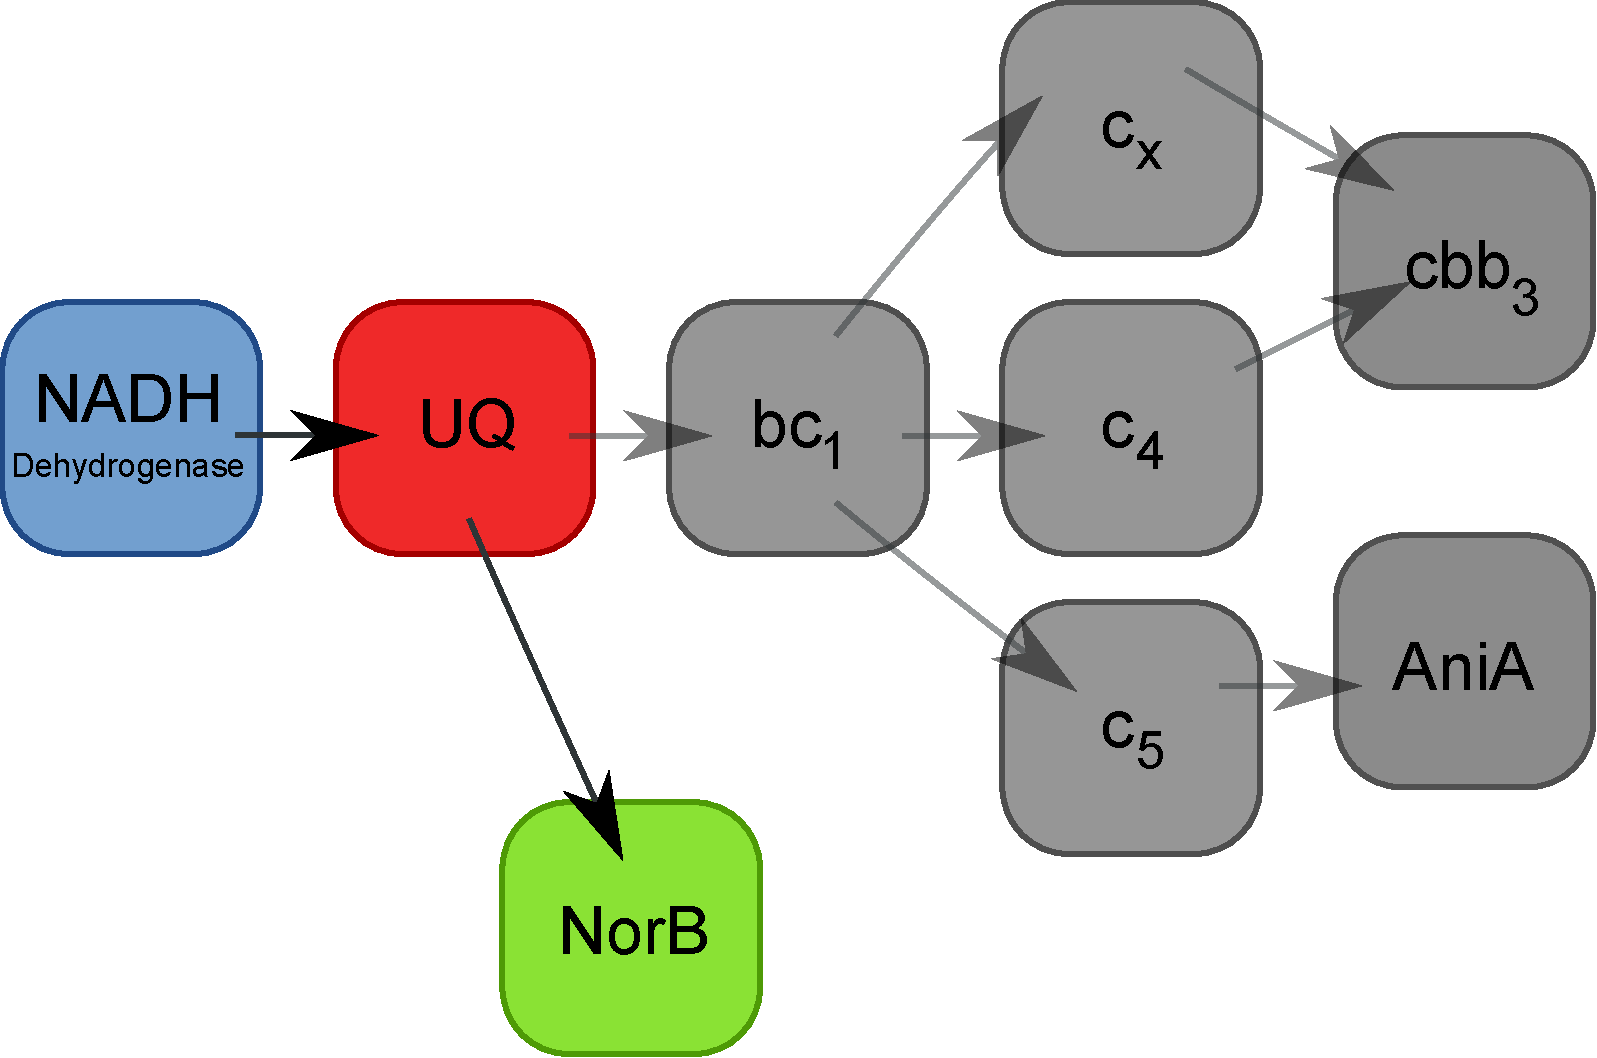
\includegraphics[width=14cm]{06-noreduction/data/no_resp_chain.pdf}
		\caption[Nitric oxide reducing electron transport chain of \Nm{}]{{\bf Nitric oxide reducing electron transport chain of \Nm{}.} This shows the complete electron transport chain of \Nsm{} with the components irrelevant to nitric oxide reduction greyed out.
	\label{fig:no_resp_chain}}
\end{figure}

These equations describe the change in concentration of Nitric Oxide over time, which is the experimentally observable value (in addition to the afore modelled oxygen). Also being modelled was the change in concentration of inhibited \cbbthree{} and the reduction state of NorB. This portion of the model involved 24 parameters and variables which I needed to estimate. This number includes the 13 values already estimated in Chapter \ref{chap:oxygenreduction}.
\subsection{Experimental Results}
Modelling nitric oxide reduction involves adding nitric oxide whilst cultures are respiring aerobically. The conditions are the same as for oxygen reduction, except that nitric oxide solution is added to a concentration of $\approx 5~\mu$M and the culture then left to respire nitric oxide.

The datasets used for this section of the model describe the effect on oxygen reduction as nitric oxide is introduced to a system that is only partially primed for microaerobic respiration. There will be a small amount of NorB (the nitric oxide reductase) present to remove and nitric oxide that is present. The $\mathit{nsrR}^-$ mutant, which expresses NorB in an essentially constitutive manner was not effective in generating a usable dataset as it removed any NO almost instantaneously resulting in an almost featureless dataset (data not shown).

The dataset and final solved output from the Monte-Carlo run are show in figure \ref{fig:nosim}. This is a more complex dataset than for oxygen respiration. Initially the oxygen reduction is carried out in exactly the same manner as the previous dataset, which is able to be modelled with the parameters selected from the prior distributions. Upon addition of nitric oxide, oxygen respiration slows and almost stops as a result of competition for electrons between \cbbthree{} and NorB, and the direct chemical inhibition of \cbbthree{} by NO. Nitric oxide starts being removed as a combination of simple diffusion (although this rate will be low) and reduction via NorB. Once the NO has been removed from the system oxygen reduction resumes at almost the same rate as before and still has the same high affinity feature as the previous dataset. The closeness of fit of the solved parameter set to the experimental data shows that the model has been able to accommodate a parameter set from the prior distributions that is able to accommodate all these features, and will still be able to model simple oxygen reduction.
\subsubsection{Prior Probability Distributions}
%lbrt
\begin{figure}[tbp]
 \centering
 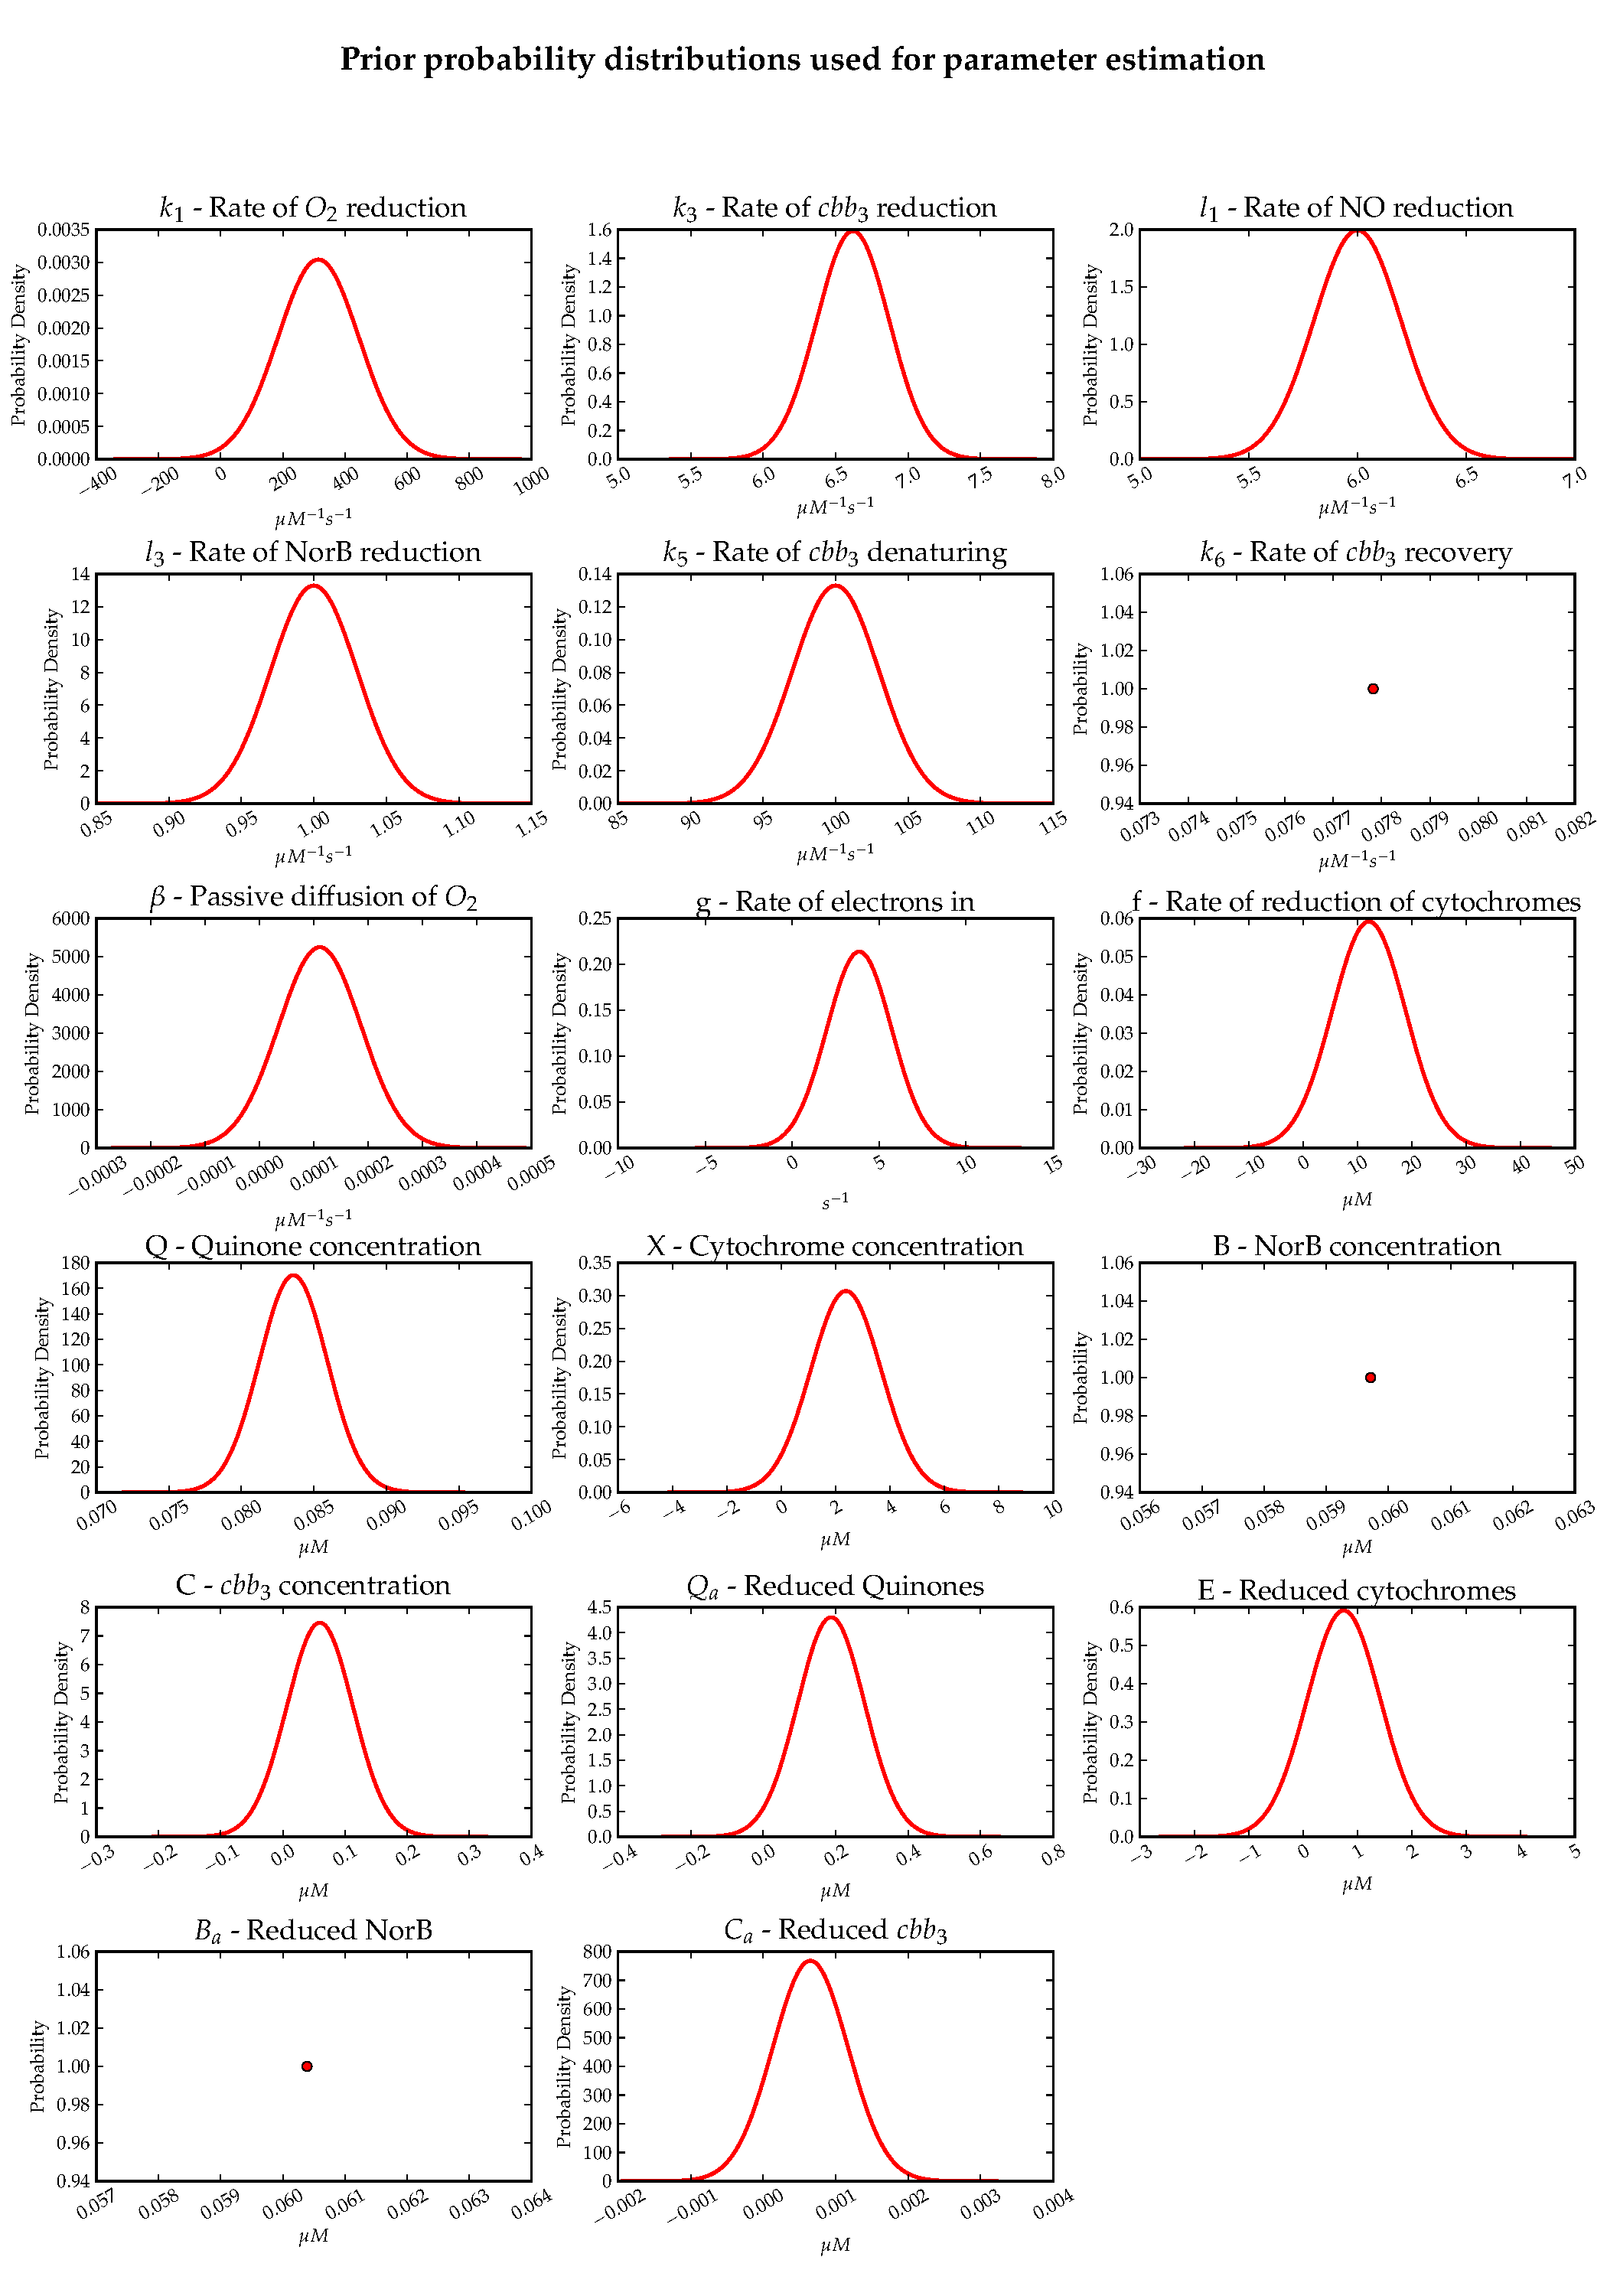
\includegraphics[width=15cm, trim=0cm 0cm 0cm 0cm]{./06-noreduction/data/aer-no-priors.pdf}
 % priors.pdf: 1008x1008 pixel, 72dpi, 35.56x35.56 cm, bb=0 0 1008 1008
 \caption[Prior probability distributions for aerobic nitric oxide reduction]{{\bf Prior probability distributions for aerobic nitric oxide reduction}. These are the probability distributions used as priors by the parameter estimation algorithm. Where no values were available in the literature, the probability distribution represents a flat prior from 0 to $\infty$ with the initial value being determined by preliminary experiment.
 \label{fig:aer_no_priors}}
\end{figure}
\subsubsection{Parameter Estimation Results}
\begin{figure}[tbp]
 \centering
 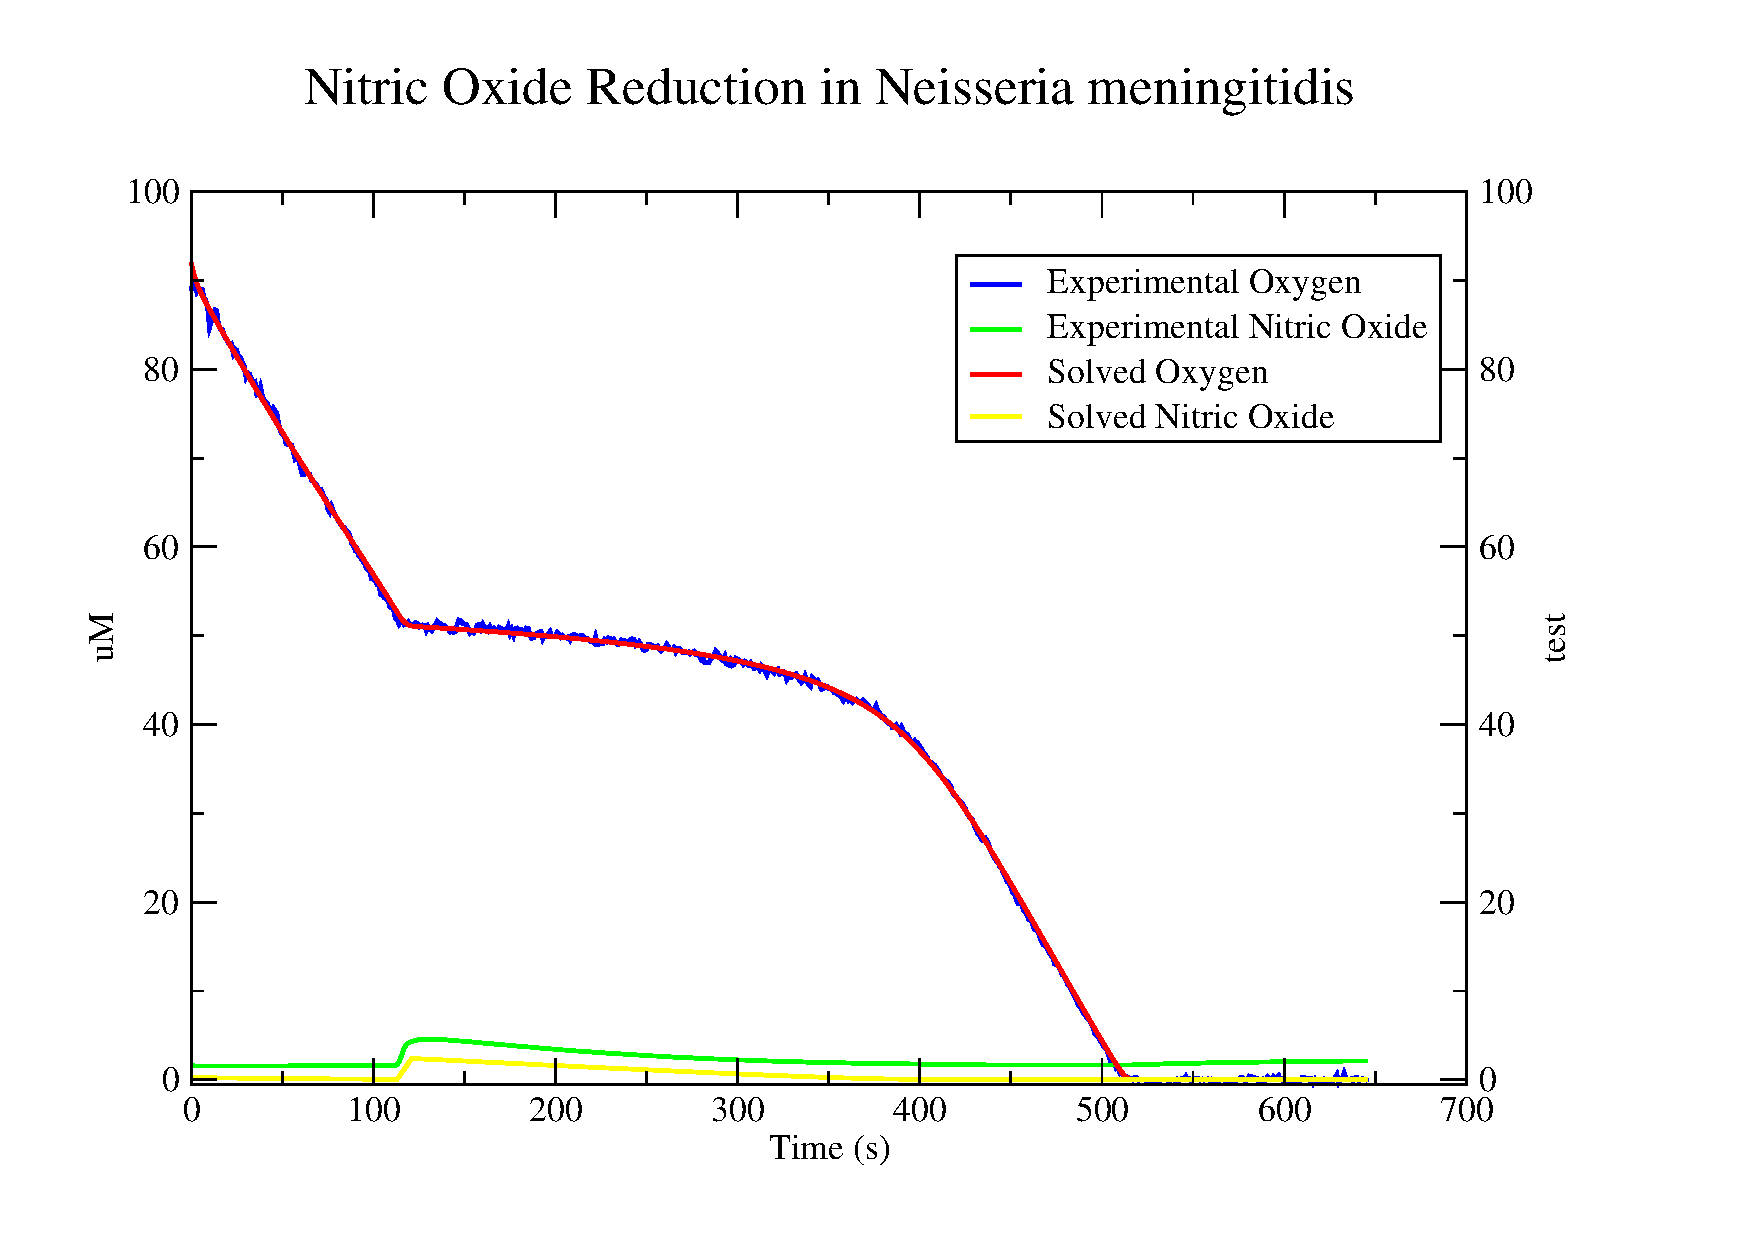
\includegraphics[width=14cm]{./06-noreduction/data/nosim.pdf}
 % nosim.eps: 0x0 pixel, 300dpi, 0.00x0.00 cm, bb=0 0 794 595
 \caption[{Nitric Oxide Reduction in \textit{Neisseria meningitidis}.}]{{\bf Nitric Oxide Reduction in \textit{Neisseria meningitidis}.} This dataset shows the effect on rate of oxygen reduction as nitric oxide is introduced to the system. The solved output, using prior probabilities from the oxygen reduction dataset show an almost perfect match to the features of the experimental dataset. The solved oxygen concentrations match the experimental dataset so closely as to be almost invisible.}
 \label{fig:nosim}
\end{figure}
\subsubsection{Analysis of Convergence}
\subsubsection{Analysis of Correlation}
\subsection{Discussion}
\section{Microaerobic Nitric Oxide Reduction}
\subsection{Introduction}
\subsection{Results}
\subsection{Discussion}
\section{\texorpdfstring{Aerobic Nitric Oxide Reduction in \textit{nsrR$^\textrm{-}$} mutant}{Aerobic Nitric Oxide Reduction in nsrR- mutant}}
\subsection{Introduction}
\subsection{Results}
\subsection{Discussion}